\section{Deterministic numerical illustrations}
\label{sec:numerics}

Figure~\ref{fig:potts-scaling} evaluates the mean-field microscopic
model with $J=1$, $\beta=4\log2$, and $a=1/2$.
Occupation triples are enumerated modulo color permutations, and
the Gamma and Beta conditional energy integrals are evaluated
analytically through their distribution functions, as derived in
Section~\ref{sec:microscopic}. Thus the plotted TV is the error
of the full spin--momentum law, not merely the spin-configuration
marginal. No Monte Carlo sampling or Gaussian approximation enters
the finite-$N$ points.

\begin{figure}[t]
 \centering
 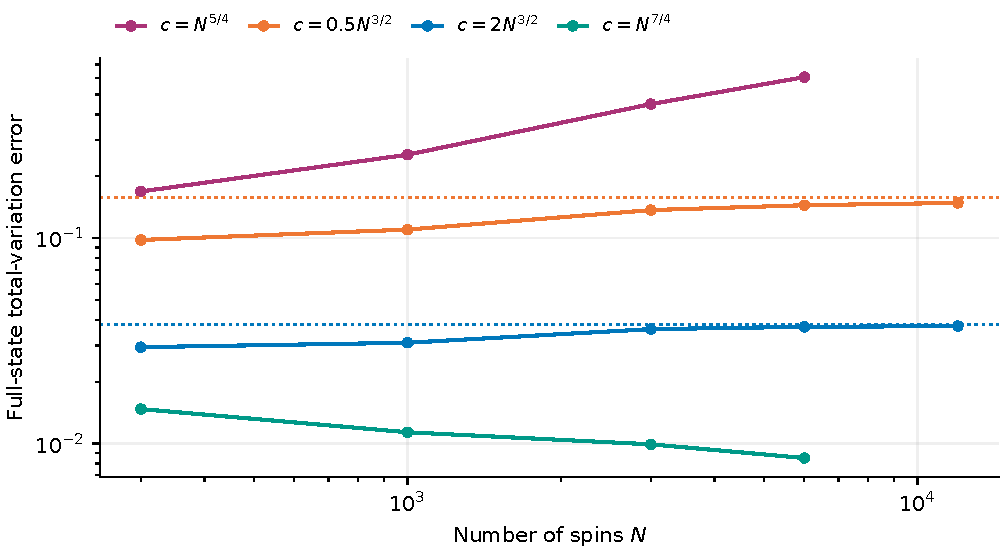
\includegraphics[width=.94\linewidth]{figures/potts-scaling.pdf}
 \caption{Exact finite-system mean-field Potts calculations with the
 physical secant bath. Points are occupation sums and Gamma/Beta CDF
 evaluations, connected to guide the eye. Dotted lines are the proved
 secant boundary limits for $c_N=\gamma N^{3/2}$, with
 $\gamma=0.5$ and $2$. The largest size, $N=12000$, was computed for
 these two boundary sequences; the other sequences extend to $N=6000$.
 These are mean-field data and do not test a short-range interfacial law.}
 \label{fig:potts-scaling}
\end{figure}

At $c_N=0.5N^{3/2}$ the predicted limit is approximately $0.157392$;
the exact $N=12000$ value is $0.148341$.
At $c_N=2N^{3/2}$ the corresponding values are $0.037986$ and
$0.037304$. These are secant-calibrated errors, not results of a
finite-$N$ optimization. The $N^{7/4}$ sequence illustrates decay
above the threshold; the $N^{5/4}$ sequence illustrates persistent
error below it. The finite range of sizes does not establish an
asymptotic exponent by itself. The theorem provides that conclusion.

These sizes are also far from the asymptotic regime of the phase
decomposition itself. The saddle of the rate function
\eqref{eq:mf-rate} at $(1/2,1/4,1/4)$ lies on the Voronoi boundary
between the ordered and disordered cells, and its rate excess is
$I(1/2,1/4,1/4)-I_{\min}=\log3-\tfrac{19}{12}\log2\simeq1.1\times10^{-3}$.
The interphase valley is therefore suppressed only by
$\exp(-0.0011N)$, which is of order one below $N\simeq10^3$.
Exact occupation sums for the pure-spin model show the slow approach.
Here Voronoi distance is Euclidean in the three occupation fractions;
ties between ordered and disordered cells are assigned to the ordered
phase. The combined ordered event is therefore $\max_j n_j\ge N/2$.
With this convention,
the Voronoi-conditional ordered variance divided by $N$ is
$1.02$ at $N=3000$ and $0.78$ at $N=12000$, against the limit
$v_-\simeq0.733$ from \eqref{eq:mf-variances}, while the ordered
weight is $0.528$ and $0.529$ against $w_-\simeq0.530$ from
\eqref{eq:mf-phase-weights}. The limiting formulas plotted as dotted
lines use the limiting constants; the finite-size points are exact.

Figure~\ref{fig:boundary-optimization} displays a different object:
the proved limiting formula for balanced phases of equal variance,
rather than microscopic finite-size enumeration.
Writing $\lambda=b\sqrt v$, preserving the phase weights gives
$2\Phi(\lambda/2)-1$, whereas optimizing the total energy gives
$\min\{2\Phi(\lambda/2)-1,1/2\}$.
The second branch is attained by abandoning one phase.
This example explains why an error report should include both the
TV value and the resulting phase populations.

\begin{figure}[t]
 \centering
 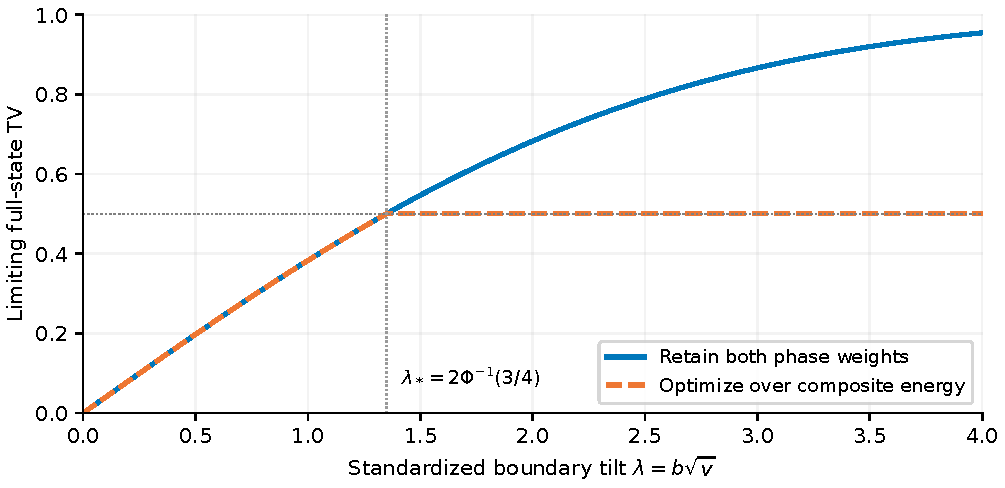
\includegraphics[width=.94\linewidth]{figures/boundary-optimization.pdf}
 \caption{The physical boundary law for balanced equal-variance phases
 under Theorem~\ref{thm:physical-boundary}'s moment and exceptional-mass
 hypotheses. This is an evaluation of the limiting formula, not
 finite-size Potts data. At
 $\lambda_*=2\Phi^{-1}(3/4)\simeq1.34898$, an optimizer that retains
 both phase populations and one that discards a phase have the same
 limiting error. The same curve holds for the exact scalar Gaussian
 model of Proposition~\ref{prop:scalar-gaussian}.}
 \label{fig:boundary-optimization}
\end{figure}

The accompanying source bundle retains the finite-system data,
figure code, and independent checks. Small systems are checked
against explicit enumeration of all $3^N$ labeled spin states for
$1\le N\le8$. At $N=12$, direct absolute-density integration verifies
the Gamma/Beta crossing formula for two kinetic shapes. Separate
normal-density quadratures verify the weighted CDF expression
\eqref{eq:physical-optimum-cdf} and its optimizer.
Floating-point calculations are numerical checks, not interval
certificates or substitutes for the proofs. The reproducibility
instructions distinguish quick checks and figure regeneration from
the more expensive full occupation enumeration through $N=12000$.
